\section{Main Functionalities}
%What are the main functionalities of the web app? what services does it offer and how it is organized?

Our web application allows users to manage potentially more than one company/economic activity, as long as they can have more than one.
Users that are logged inside the webapp can modify their companies data, and also bank accounts linked to them.
Furthermore, users can perform CRUD operations on their own products/services by their own catalogues, and also of their customers. Users can also
extract lists of their products and their customers in a PDF file.
Coming to the main part, users can decide to "open" a new invoice to a specific customer: once the user decide to bill, the invoice become closed
and no longer editable; a PDF warning is produced and sent to the customer: when payment is performed, by a button the actual invoice in both
formats (PDF as courtesy for the customer, XML for the italian system "SISTEMA DI INTERSCAMBIO") is printed out.
Concluding, notifications are sent through telegram and / or email, as specified by the user in his preferences, and insight charts are available to
him providing many information, as for example which customers revenue to the company in a specified time slot.

In particular, our web application is divided in four main parts:
\begin{itemize}
    \item User Management: users do not have the possibility to register on the web application: this is due to the fact that the application is designed to be deployed on a specific container (taking advantage of virtualization technologies) for each customer: in this scenario, a single owner user is setted up manually. Moreover, the user is not allowed to create companies, as long for each company managed a license is required. Users can edit their data, data of their companies and of their bank accounts. Users can switch the company currently used in the application by selecting it from a dropdown menu always accessible in all pages of the web application.
    \item Business Management (the core part of the application): users can perform CRUD operations on customers and products linked to each of their companies, and getting lists of them both through the web application and in PDF format. They can create new invoice entities: an invoice in the early stages of creation has to be considered like an "open debt" to the customer to which the invoice is related: at the very first stage, in fact, the invoice is empty but from that moment, users can start to add rows to the invoice, that correspond to specific sellings, and that will appear on the final invoice as a detail row. Whenever the user decide to bill the invoice, that will become immutable, a document in PDF format will be provided to the user and sent to the customer that will able to perform the payment. Once that the payment has been performed by the customer, the user can emit the actual invoice in XML format that complies with italian regulations. This implementation also complies with the italian legislation, as long a company has 14 working days to submit the invoice to the SDI (Interchange System) before encountering sanctions, and so the invoice can be actually printed out after the payment.
    \item Notification Management: notifications are directed both to the user and to customers: for what concerns the user, he has the opportunity to get them both via mail and via Telegram. He can set up these preferences on his reserved area, as long as for telegram is also needed to specify his Chat ID. notifications for customers are only via mail. /*when are performed?*/
    \item Insight Printout: the user has the possibility to see, for each company, different typologies of insight plots, as for example histograms on invoices in a certain amount of time, sales in a certain amount of time, invoices filtered by customers, sales filtered by customers, total discount for a certain amount of time.
\end{itemize}

\subsection{Deployment - CI/CD}\label{subsec:deployment---ci/cd}
In Bitbucket, Pipelines is a powerful feature that automates the build, test, and deployment process of your code.
It's a continuous integration and delivery (CI/CD) tool that helps you streamline your development workflow and ensure that your code is always up-to-date and error-free.
Our pipeline consists of two essential steps.
The first step is the build phase, which is responsible for compiling the code, This step helps us identify any errors or issues in our code early on, preventing unwanted errors from occurring in the future.
If the build phase passes successfully, the next step is the deployment phase.
This step deploys the latest version of our code to our server, ensuring that our application is always up-to-date and running smoothly.
With Pipelines, we can easily monitor the progress of our builds and deployments, and quickly troubleshoot any issues that may arise.

\begin{figure}[h!]
    \centering
    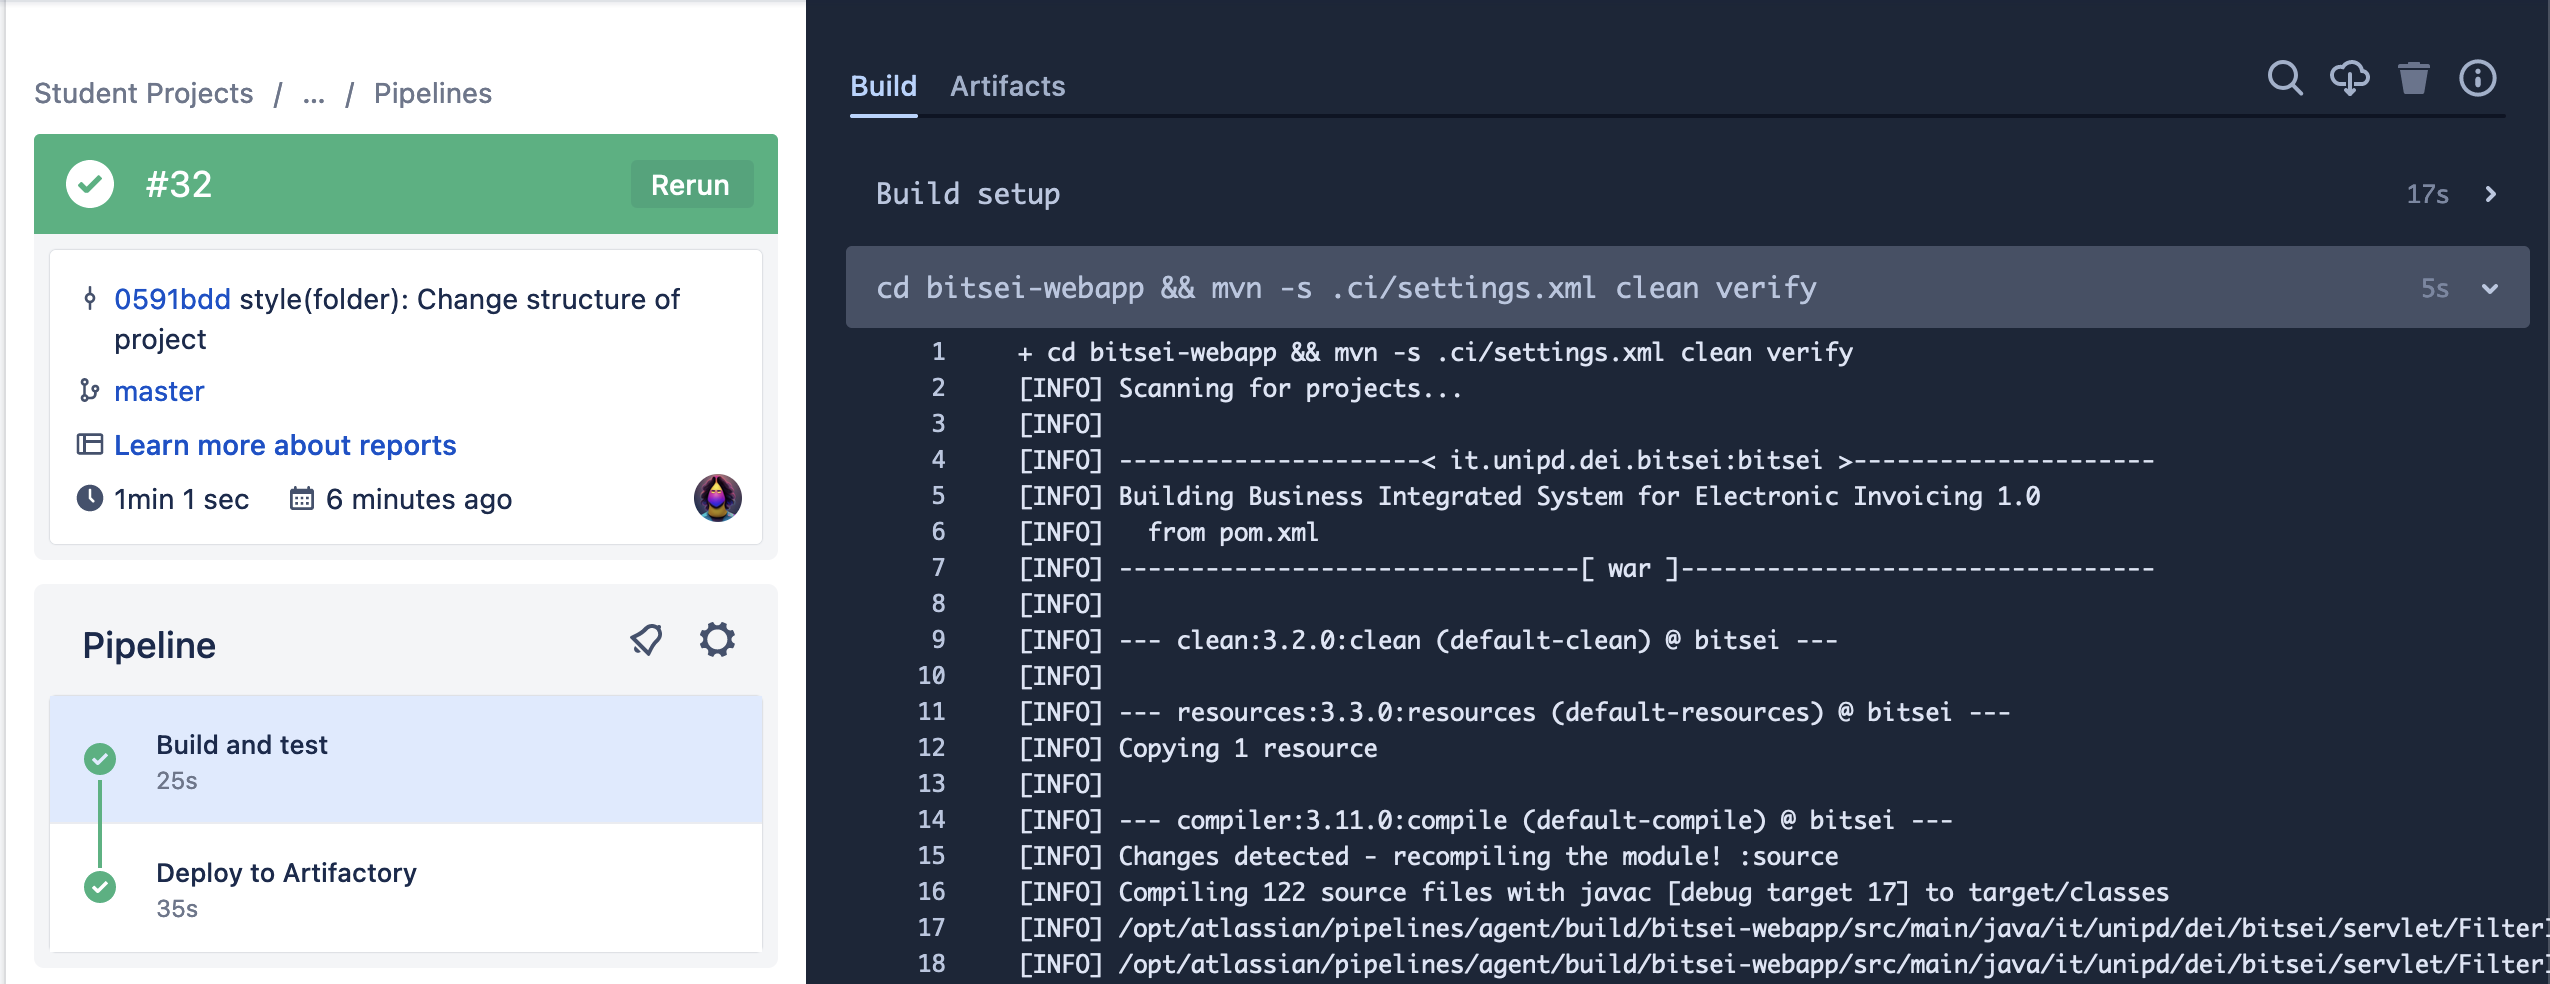
\includegraphics[height=390pt, keepaspectratio]{resources/pipeline.png}\label{fig:bitbucket-pipeline}
\end{figure}